%
\documentclass[runningheads]{llncs}

% Add plot library
\usepackage{graphicx}
\usepackage{pgfplots}
\usepackage{pgf-pie}
\usepackage{caption}
\usepackage{subcaption}
\usepackage{adjustbox}
\usepackage{hyperref}

% Define colors
\definecolor{darkblue}{HTML}{264653}
\definecolor{blue}{HTML}{2a9d8f}
\definecolor{green}{HTML}{8ab17d}
\definecolor{yellow}{HTML}{e9c46a}
\definecolor{orange}{HTML}{f4a261}
\definecolor{red}{HTML}{e76f51}

\begin{document}
\pgfplotsset{compat=1.18}

\title{Relevance in Reference Recommendation by LLMs: A Meta-Analysis}
%
%\titlerunning{Abbreviated paper title}
% If the paper title is too long for the running head, you can set
% an abbreviated paper title here
%
% \author{Domonkos Kostyál \and Tanguy Lissenko \and Théo Fuhrmann}

\institute{Music Technology Group, Universitat Pompeu Fabra, Barcelona, Spain
% \email{domonkos.kostyal01@estudiant.upf.edu}\\
% \email{tanguy.lissenko01@estudiant.upf.edu}\\
% \email{theo.fuhrmann01@estudiant.upf.edu}
}
%
\maketitle

\begin{abstract}

Large Language Models (LLMs) are increasingly used in academic research, including for the task of recommending relevant references. However, there are concerns about the accuracy and relevance of LLM-generated citations. This meta-analysis examines the performance of three state-of-the-art LLMs – Chat-GPT, Claude, and Gemini – in recommending relevant scientific papers for 6 research topics with 3 subcategories each in music and sports. Relevance is assessed based on the hallucination rate, publication date, citation count, and topic alignment. The findings reveal that Chat-GPT exhibits the highest citation accuracy (63.3\%), but all three models struggle with nuanced citation tasks, sometimes recommending non-existent or irrelevant papers. The results suggest that LLMs can be valuable tools for reference recommendation, but researchers should exercise caution and critically evaluate LLM outputs to ensure accuracy and relevance. Further research should explore the impact of model-specific training data and internet access capabilities on reference recommendation performance.


\keywords{Meta-research \and Relevance \and Artificial intelligence \and Large Language Models \and Chat-GPT \and Claude \and Gemini}
\end{abstract}

\section{Introduction}

%Background of the problem (motivation)  
References are the fundamentals of quality research.
Therefore, to find relevant papers on a  topic is crucial for several key reasons. Most importantly they help to establish credibility, contextualize your contributions and acknowledge prior works. They also have an essential role in providing ideas to a research task.

%Why it is important, interesting  
Traditional methods of obtaining references include the use of specialized search tools such as google scholar, arXiv or others.
These methods are often tedious and time consuming for researchers as the databases for a particular domain can be massive and the selected articles are not always relevant.

In recent years the emergence of AI assistants, especially LLMs have helped people in several aspects of their life. Researchers have also drawn their attention to LLMs to incorporate it in their work for various tasks. 
One task for which LLMs can be useful is for that problem of collecting references for a particular subject, such as scientific articles, theses or books.
But there are potential risks in using LLMs for this purpose. The risks may be that the references given are not real, partially correct, irrelevant to the subject, etc.

%What others have done to solve the problem (all related existing work should be %described and referenced) 
Therefore, in order to make the best use of LLMs for the reference collection, previous research has investigated and quantified the potential risks of an uninformed use.
Past work has focused largely the accuracy of the bibliographic citations provided by Chat-GPT \cite{Chat-GPT2024}.
Earlier research on early models of Chat-GPT was more pessimistic about the accuracy of the results obtained \cite{day2023}. Precision was evaluated on the basis of criteria such as title, authors, journal name, etc.
However, more optimistic results were obtained when considering more recent, high-performance versions of Chat-GPT \cite{byun-etal-2024-reference,walters_2023}.

%Brief description of the proposed solution  
Our research compares models that have not been compared in the past: Chat-GPT 4o, Claude 3.5 Sonnet and Gemini 1.5 Flash. The relevance of the results obtained is judged on the basis of the percentage of hallucination rate (references that do not exist), the date of publication, the journal impact factor (JIF) and the number of citations.
 We also make a comparison on the basis of different topics, which we subdivide into three categories corresponding to a notion of domain complexity, quantified by the number of publications published for this topic.

We start with a review of the literature, examining what has already been done on the subject. Then we explain our methodology, which is based on a common prompt that we submit to the various models we study. This is followed by an explanation of our results, based on an analysis of the database obtained during the experiment. We conclude with a discussion of our method, results and future directions.

%Last paragraph, summarizes somehow what will be described in each section of the %paper

\subsection{Literature Review}\label{literature}

Many citation recommendation systems already exist, each employing distinct methods. Färber et al. \cite{farber_2020} highlights this diversity by reviewing previously used approaches. Early methods were based on hand-crafted features, but, as he notes, \textit{"In recent years, no novel approaches of this group have been published any more..."}. This shift occurred because deep learning techniques now consistently outperform these traditional models. Färber et al. also discuss methods like topic modeling, machine translation, and neural networks.

Jevin D. West et al. \cite{jevin_2016} propose a solution using hierarchical clustering. They first rank all papers using a unique algorithm called article-level Eigenfactor, then apply clustering to the results. Some approaches, as noted by Renuka, S. and Raj Kiran \cite{Renuka_2021}, leverage Natural Language Processing (NLP) to process and classify articles more comprehensively compared to traditional approaches.

The use of large language models (LLMs) has expanded from everyday life into research fields as well. Nitin et al.'s study \cite{Rane_2023} explores Chat-GPT’s applications across various academic disciplines, examining how LLMs can enhance learning experiences and streamline administrative tasks, while also addressing critical issues related to bias, ethics, and data privacy.

However, as the role of AI in research grows, concerns about over-reliance are also increasing. Buçinca et al. \cite{buccinca_2021} warn that AI’s presence in decision-making can lead to \textit{“automation bias”} where researchers accept AI outputs uncritically, potentially bypassing critical literacy skills in favor of AI convenience. This dependence risks diminishing the researcher’s role in actively interpreting and validating data findings, which is fundamental to rigorous scientific inquiry. 

We identified two significant studies closely related to our research, making it worthwhile to examine their findings in detail. The first research conducted by Byun et al. \cite{byun-etal-2024-reference} and the second is authored by Chelli et al. \cite{Chelli_2024}. Byun compared the accuracy of different GPTs, with the latest, GPT-4. Their method involved providing Chat-GPT with titles and abstracts of existing papers and requesting related works. They tested three different prompts and evaluated them separately. The prompt that yielded the most comparable results in their study was the one in which they asked for only references:

\textit{"You are an [NLP or HCI] researcher working on a paper to submit to [EMNLP or CHI]. 
The paper you are working on is titled: [PAPER TITLE] The abstract for your paper is: [PAPER ABSTRACT]
List 10 relevant papers you could cite in your Related Works section. Write each citation in APA format."}

With this query, they collected twenty papers from two different venues (HCI, NLP), their final dataset had 1616 annotated citations. Their total accuracy in the titles was 66\% and the precision of authors was 88.64\% using GPT-4. However, while these accuracy rates offer valuable insights into the technical capabilities of GPT-4, they do not address whether the recommended citations are genuinely relevant to the specific context and needs of each research topic, a limitation that remains to be investigated. If we compare these to Chelli's results which is in general just a brief overview focusing on medical fields, they collected similar results from 471 citations: The hallucination rate was 28.6\% for GPT-4. They also evaluated Bard (the older version of Google Gemini) and their result was 91.4\%. To convert their metrics to accuracy we just need to extract them from 1, so respectively 71.4\% and 8.6\% which is comparable to Byun's result.

We can see that previous research has largely concentrated on metrics tied to information accuracy. Although understanding accuracy is essential, accurate citations that lack relevance remain unhelpful for researchers. In this study, we continue to evaluate accuracy, but we also provide an initial evaluation of the relevance of citations identified by the three aforementioned models.

\section{Research methodology}

%Explain the research methodology that you propose to be applied in order
%to achieve the research goal. Justify the selection of the methodology
%and why other methods are discarded. You may want to include references
%supporting your arguments in the selection of the methodology, and
%describing the methods proposed. Explain the strengths and limitations
%of the proposed research methodology applied. You can use figures or
%tables to illustrate the phases of the research methodology, indicate
%the data gathering techniques, different data types considered, etc., if
%appropriate. This section can be of ¾ or 1 page long.

To systematically evaluate the relevance of scientific paper recommendations by LLMs, we designed a consistent prompt schema to be used across all tested models. The prompt schema aimed to simulate an academic inquiry for relevant research articles, following the format:

\textit{“I'm writing a research paper on X. To get me started, give me five relevant scientific papers on the topic. Include the authors and published date. Don’t include a summary of the article.”}

where X is the field of study or specific topic of interest.

\subsection{Fields of study}

We selected two broad categories, sports and music, to introduce diversity and to avoid focusing solely on a single subject area. Within each category, we chose three topics that represent a gradient of specificity (broad, medium and narrow): For music: Music, Rock Music, and Shoegaze. For sports: Sports, Basketball, and Basketball Shooting Technique.

To ensure relevance in recommendations, we deliberately chose topics that are well-established rather than cutting-edge, which allows us to observe whether the LLMs prioritize recommending foundational or highly regarded works over recent publications that may not yet have proven significance.

In order to objectively assess topic specificity, we collected the number of search results for each topic on Google Scholar and JSTOR. These results provided an indication of the information availability and topic breadth, supporting our categorization from general to highly specific topics. The following figure serves to visually justify the specificity levels and highlights how fewer resources exist as topics become more narrowly focused.

\begin{figure}
    \centering
    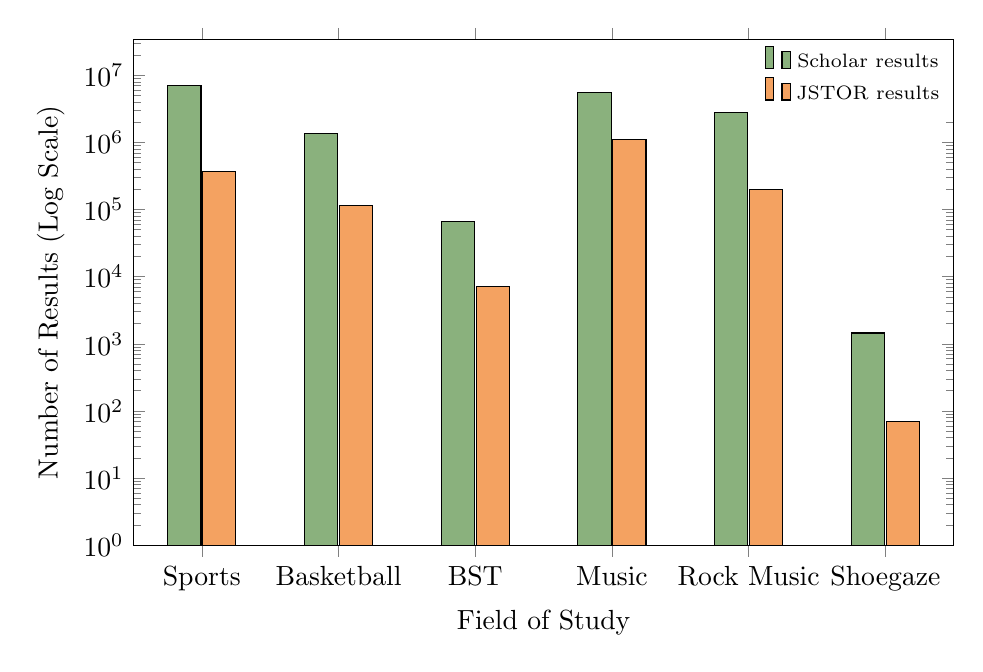
\begin{tikzpicture}
        \begin{axis}[
            ybar=0.6pt,
            bar width=12pt,
            width=12cm,
            height=8cm,
            enlarge x limits=0.1,
            symbolic x coords={Sports, Basketball, BST, Music, Rock Music, Shoegaze},
            xtick=data,
            ylabel={Number of Results (Log Scale)},
            xlabel={Field of Study},
            ymode=log,
            ymin=1, % Start at a minimum of 1 to handle log scale correctly
            log origin=infty,
            legend style={at={(1,1)}, anchor=north east, draw=none, font=\scriptsize},
        ]
            % Scholar results in darker gray
            \addplot[fill=green] coordinates {(Sports, 7000000) (Basketball, 1370000) (BST, 65700) (Music, 5620000) (Rock Music, 2770000) (Shoegaze, 1450)};
            
            % JSTOR results in lighter gray
            \addplot[fill=orange] coordinates {(Sports, 372821) (Basketball, 115125) (BST, 7238) (Music, 1093996) (Rock Music, 195885) (Shoegaze, 69)};
            
            \legend{Scholar results, JSTOR results}
        \end{axis}
    \end{tikzpicture}
    \caption{Number of search results in the Scholar and JSTOR databases. BST refers to Basketball Shooting Technique}
\end{figure}

This setup allowed us to test each LLM’s ability to maintain relevance in recommendations across varying degrees of topic specificity.

\subsection{Data collection}

For each LLM response, we collected the following information to evaluate the relevance of the suggested articles:

\begin{itemize}
    \item \textbf{Verification of Existence:} We first verified if the recommended articles existed. Petiska \cite{petiska_2023} observed that Chat-GPT often relies on Google Scholar citation counts when suggesting citations. Therefore, we searched Google Scholar for each paper, and if not found there, we attempted to locate it through regular internet search. For each verified paper, we analyzed the accuracy of the \textbf{title}, \textbf{authors}, and \textbf{publication date}.
    \item \textbf{Publication date:} Recency is important for relevance, as recent works often reflect the latest developments. Modern search engines prioritize new publications, but older influential works can also be highly relevant, especially in well-established fields. Dong et al. \cite{dong2010towards} emphasize that both recency and reliability affect trust and relevance in information retrieval.
    \item \textbf{Citation Count:} The citation count reflects a paper's relevance and recognition within the scientific community, as a higher number of citations often indicates greater academic impact. According to Bornmann \cite{bornmann2017measuring}, the frequency with which a paper is cited demonstrates its significance and influence. However, it's important to note that more recent papers are less likely to have high citation counts due to their recency, despite potentially being highly relevant in a specific field.
    \item \textbf{Journal Category Relevance and Impact Factor:} The relevance of a journal to the research topic is crucial in determining whether a paper contributes meaningfully to the field. Journals that align with the specific research area ensure that the recommended papers are contextually appropriate. Additionally, the Impact Factor of a journal reflects its overall academic influence and credibility, serving as a measure of the journal's reputation and the quality of the research it publishes. Pagani et al. \cite{pagani2015methodi} used a combination of impact factor, publication year, and citation count as crucial features for developing a relevance ranking method, underscoring the importance of these factors in assessing academic relevance.
\end{itemize}

The collected features provided a framework for quantifying the relevance of each recommendation. Together, they allowed us to assess the models’ effectiveness in providing high-quality academic resources for both broad and highly specific topics.

\subsection{LLM features}

To contextualize the performance of each LLM, we documented relevant characteristics, including the model version, knowledge cutoff date, and internet access capabilities. These factors may influence the LLMs’ recommendation accuracy and relevance, particularly when addressing topics that require up-to-date or lesser-known information.

\begin{table}[!ht]
    \centering
    \begin{tabular}{c c c c}
        \hline
        \textbf{LLM} & \textbf{Version} & \textbf{Internet Access} & \textbf{Knowledge cutoff} \\
        \hline
        Chat-GPT & 4o & Yes & October  2023\footnotemark[1] \\
        Claude & 3.5 Sonnet & No & April 2024\footnotemark[2] \\
        Gemini & 1.5 Flash & Yes & N/A\\
        \hline
    \end{tabular}
    \caption{LLM characteristics.}
\end{table}

\footnotetext[1]{Source: OpenAI Documentation, available at \url{https://platform.openai.com}}
\footnotetext[2]{Source: Anthropic Model Card, available at \url{https://assets.anthropic.com}}


These model-specific features were recorded to allow for deeper insights into each model’s capacity to generate relevant paper recommendations across a spectrum of topic specificity.

\section{Results}\label{results}

\subsection{Hallucination rate}

Once the data has been collected, we commence with generally verifying the accuracy of the recommended articles. This has been made before, although only with older versions of LLMs mostly focusing on Chat-GPT. Therefore, this can be an interesting comparison with previous research, showing whether they have improved or not. 

% Pie Charts Matrix without labels and captions
\begin{table}[!h]
\centering

\begin{tabular}{c|ccc}
\hline
\rotatebox{90}{\textbf{}} & \textbf{Chat-GPT} & \textbf{Claude} & \textbf{Gemini} \\
\hline
\rotatebox{90}{\textbf{Broad}} & 
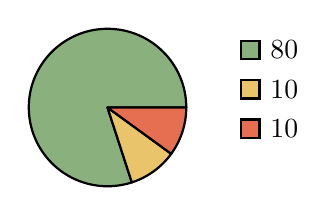
\begin{tikzpicture}
    \pie[hide number, radius=1, color={green, yellow, red}, text=legend] {80,10,10}
\end{tikzpicture} &
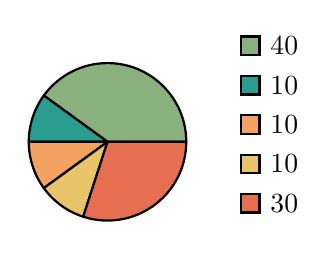
\begin{tikzpicture}
    \pie[hide number, radius=1, color={green, blue, orange, yellow, red}, text=legend] {40, 10, 10, 10, 30}
\end{tikzpicture} &
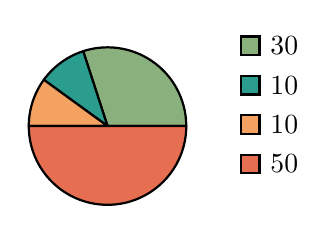
\begin{tikzpicture}
    \pie[hide number, radius=1, color={green, blue, orange, red}, text=legend] {30, 10, 10, 50}
\end{tikzpicture} \\
\hline
\rotatebox{90}{\textbf{Medium}} & 
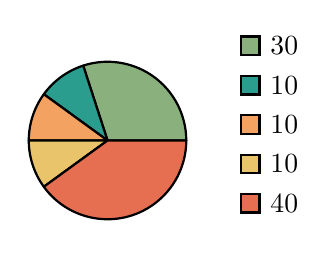
\begin{tikzpicture}
    \pie[hide number, radius=1, color={green, blue, orange, yellow, red}, text=legend] {30, 10, 10, 10, 40}
\end{tikzpicture} &
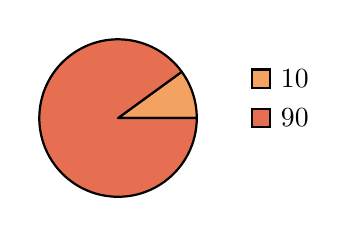
\begin{tikzpicture}
    \pie[hide number, radius=1, color={orange, red}, text=legend] {10, 90}
\end{tikzpicture} &
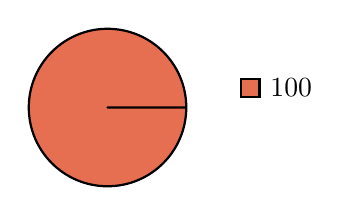
\begin{tikzpicture}
    \pie[hide number, radius=1, color={red}, text=legend] {100}
\end{tikzpicture} \\
\hline
\rotatebox{90}{\textbf{Narrow}} & 
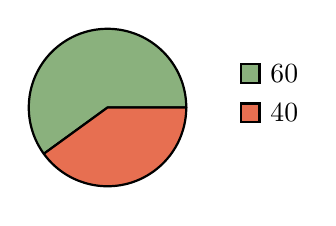
\begin{tikzpicture}
    \pie[hide number, radius=1, color={green, red}, text=legend] {60,40}
\end{tikzpicture} &
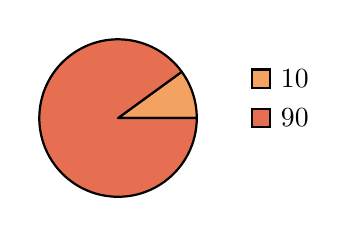
\begin{tikzpicture}
    \pie[hide number, radius=1, color={orange, red}, text=legend] {10,90}
\end{tikzpicture} &
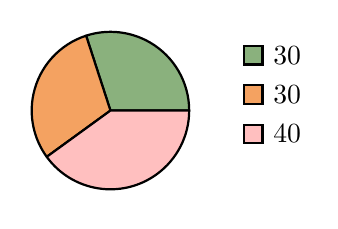
\begin{tikzpicture}
    \pie[hide number, radius=1, color={green, orange, pink}, text=legend] {30, 30, 40}
\end{tikzpicture} \\

\hline
\hline
\rotatebox{90}{\textbf{Total}} & 
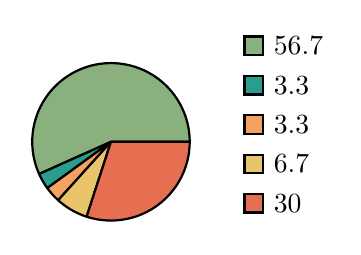
\begin{tikzpicture}
    \pie[hide number, radius=1, color={green, blue, orange, yellow, red}, text=legend] {56.7,3.3, 3.3, 6.7, 30}
\end{tikzpicture} &
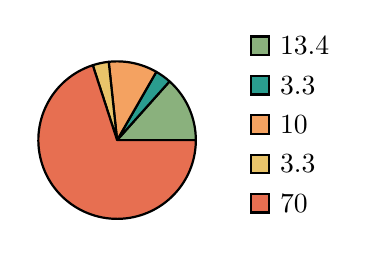
\begin{tikzpicture}
    \pie[hide number, radius=1, color={green, blue, orange, yellow, red}, text=legend] {13.4, 3.3, 10, 3.3, 70}
\end{tikzpicture} &
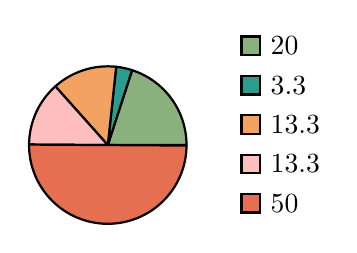
\begin{tikzpicture}
    \pie[hide number, radius=1, color={green, blue, orange, pink, red}, text=legend] {20, 3.3, 13.3, 13.3, 50}
\end{tikzpicture} \\
\end{tabular}

\parbox{\textwidth}{
    \centering
    \textcolor{green}{\rule{10pt}{10pt}} \textbf{Correct} \quad
    \textcolor{blue}{\rule{10pt}{10pt}} \textbf{Confused 2 papers} \quad
    \textcolor{orange}{\rule{10pt}{10pt}} \textbf{Wrong author} \quad
    \\
    \textcolor{yellow}{\rule{10pt}{10pt}} \textbf{Wrong title} \quad
    \textcolor{pink}{\rule{10pt}{10pt}} \textbf{Web article} \quad
    \textcolor{red}{\rule{10pt}{10pt}} \textbf{Not Existent}
}
\caption{Results overview for different topic levels}
\label{table:hallucinations}
\end{table}

Our results can be seen in table \ref{table:hallucinations}. The following list provides a detailed description of the used labeling for clarification:

\begin{itemize}
    \item \textbf{Correct:} The article is existent and it is referenced correctly.
    \item \textbf{Confused 2 articles:} On rare occasions it confused two articles which have the same title and it mixes up the authors.
    \item \textbf{Wrong author:} These were the situations where the title was correct, but at least one of the authors was incorrectly identified. In these cases sometimes the publication year was also wrong but this wasn't in our focus.
    \item \textbf{Wrong title:} These were the scenarios when only the title had some false modification. For example the authors and year were correct but the title had a small variation.
    \item \textbf{Web article:} This is made specifically for Gemini, as it sometimes recommended web pages instead of academic papers, which were requested.
    \item \textbf{Not Existent:} It's impossible to identify the recommended paper.
\end{itemize}

To get a better understanding of the general accuracy of each model, it's a good method if we check all the title's accuracy, whether they existent or not. It is visible (table \ref{table:title_acc}), that Chat-GPT outperformed all of the models. Interestingly, Gemini demonstrated a level of accuracy comparable to Chat-GPT in the narrow topic case, although more than half of its recommendations consisted of web articles. If we compare these results to previous researches, both Byun (88.64\% with GPT-4) and Chelly (71.4\%) addressed better ratios. This could be attributed to the limited size of our dataset and the narrow range of topics. Gemini showed a significant improvement, increasing from Chelly’s 8.6\% (with Bard) to 36.7\%. However, this remains only half the performance rate achieved by GPT-4o.

Similar results are observed in the authors’ accuracy (Table \ref{table:author_acc}), where Chat-GPT achieved an accuracy of 90.6\%, closely aligning with Byun’s results. Meanwhile, Claude and Gemini showed comparable performance, each reaching approximately 60\%.

\begin{table}[ht]
    \footnotesize
    \centering
    \begin{minipage}{0.45\textwidth}
        \centering
        \begin{tabular}{ l c c c }
            \hline
             & \textbf{Chat-GPT} & \textbf{Claude} & \textbf{Gemini} \\
            \hline
            Broad & 80\% & 60\% & 50\% \\
            Medium & 50\% & 10\% & 0\% \\
            Narrow & 60\% & 10\% & 60\% \\
            Total & 63.3\% & 26.7\% & 36.7\% \\
            \hline
        \end{tabular}
        \caption{Title accuracy}
        \label{table:title_acc}
    \end{minipage}
    \hfill
    \begin{minipage}{0.45\textwidth}
        \centering
        \begin{tabular}{ l c c c }
            \hline
             & \textbf{Chat-GPT} & \textbf{Claude} & \textbf{Gemini} \\
            \hline
            Total & 90.6\% & 55.6\% & 66.8\% \\
            \hline
        \end{tabular}
        \caption{Author accuracy}
        \label{table:author_acc}
    \end{minipage}
\end{table}

On table \ref{table:hallucinations}, we wanted to separate when the model confused two articles or just made up the authors. This phenomenon presents a problem due to the inherent nature of LLMs and how they train on datasets. It's model independent, although it mostly occurred when the topic was more general.

In spite of our expectations, there wasn't significant decrease in accuracy when we narrowed down the topics. Only Claude showed the closest behavior, however it performed the worst probably due to the lack of web access. On the other hand, Gemini also recommended some websites with relevant articles, despite our prompt explicitly requesting research papers. In our case, this was acceptable because we focused on general topics to gain a broader understanding of a field of study.

Surprisingly, the "middle" query, which were the rock music and basketball topics, performed the worst. Claude nearly hallucinated all of its responses, finding only one relevant source. However, Gemini did even worse, fabricating articles in both fields entirely. 

%\subsection{Relevance}
%\subsection{Article features}
%\subsubsection{Titles}

\subsection{Publication Years}

Figure~\ref{fig:year_box_plot} illustrates the distribution of citation years for bibliographic references retrieved by the three LLMs. Each box plot provides an overview of the spread of publication years.
Chat-GPT was assessed using 22 published, non-fiction articles. Claude's evaluation was based on 8 published, non-fiction articles, and Gemini was assessed with 20 published, non-fiction articles.
For Chat-GPT, the median publication date is 2015, with the inter-quartile range spanning from 2008 to 2023. This distribution indicates a potential preference for more recent sources, as the second quartile falls in 2023 and the maximum year reaches 2024.
For Claude, the median publication date is 2013, with the inter-quartile range between 2010.5 and 2014. This suggests a tendency toward older sources, as the second quartile is 2014 and the maximum year is 2015.
For Gemini, the median publication date is 2001, with the inter-quartile range from 2008 to 2020. This distribution points to a broader coverage of sources from various time periods.
Chat-GPT and Gemini exhibit greater variability in publication years, as indicated by their higher standard deviations around the mean (13.8 and 7.25), whereas Claude shows lower variability with a smaller standard deviation (2.4).

\subsection{Number of Citations}

Figure~\ref{fig:citations_box_plot} illustrates the distribution of citations numbers for bibliographic references retrieved by the three LLMs.
Chat-GPT was assessed using 22 published, non-fiction articles. Claude's evaluation was based on 8 published, non-fiction articles, and Gemini was assessed with 15 published, non-fiction articles.
Chat-GPT has a median citation number of 59.5 with the inter-quartile range spanning from 1.0 to 177.5. The standard deviation is 460.
Claude has a median citation number of 160 with the inter-quartile range spanning from 135 to 860.5. The standard deviation is 510.82.
Gemini has a median citation number of 18 with the inter-quartile range spanning from 5 to 1455.5. The standard deviation is 1606.35.
From our results we find that Gemini has the highest citation counts and the highest variability while Chat-GPT has the lowest average and a wider range of citation numbers.
Claude's citation counts are more concentrated around the median, with fewer extreme values.

\subsection{Journal Impact Factor}

Figure~\ref{fig:jif_box_plot} illustrates the distribution of journal impact factors for bibliographic references retrieved by the three LLMs.
Chat-GPT was assessed using 18 published, non-fiction articles. Claude's evaluation was based on 6 published, non-fiction articles, and Gemini was assessed with 5 published, non-fiction articles.
Chat-GPT has a median JIF of 2.9 with the inter-quartile range spanning from 2.3 to 2.975. The standard deviation is 2.3.
Claude has a median JIF 2.4 with the inter-quartile range spanning from 1.9 to 2.975. The standard deviation is 3.5.
Gemini has a median JIF of 3.7 with the inter-quartile range spanning from 0.9 to 3.9. The standard deviation is 3.55.

\begin{figure}[htbp]
    \centering
    % Subfigure A
    \begin{subfigure}[b]{0.32\textwidth}
        \centering
        \includegraphics[width=\linewidth]{figures/years_box_plot.png}
        \caption{Year Box Plot}
        \label{fig:year_box_plot}
    \end{subfigure}
    % Subfigure B
    \begin{subfigure}[b]{0.32\textwidth}
        \centering
        \includegraphics[width=\linewidth]{figures/citations_box_plot.png}
        \caption{Citations Box Plot}
        \label{fig:citations_box_plot}
    \end{subfigure}
    % Subfigure C (below)
    \begin{subfigure}[b]{0.32\textwidth}
        \centering
        \includegraphics[width=\linewidth]{figures/jifs_box_plot.png}
        \caption{JIF Box Plot}
        \label{fig:jif_box_plot}
    \end{subfigure}
    
    \caption{Year box plot, Citations box plot and JIF box plot}
    \label{fig:grouped_figures}
\end{figure}

\subsection{Journal Categories}

The last feature we analyzed was the journal categories using the tables ~\ref{tab:sports_topics} and ~\ref{tab:music_topics}. Starting with Chat-GPT, we can observe a more generalist behavior in the Sports, Shoegaze and BST topics. However, it introduced journals with more diversity in Basketball, Music and Rock Music. As for Basketball and Music, not only it explored interesting related categories such as biology, education and mathematics, but it identified exact topic matches, recommending "sports sciences" and "music" respectively.

In contrast, Claude had more specialized categories. It showed very relevant and varied categories for the Sport category. Moreover, it identified the matching topic for BST. As for the musical topics, it showed special focus in biology for Music and psychology for Basketball.

Gemini obtained a mix of specialized and generalist categories. It found relevant categories for Sports focusing more on medical fields. It also identified the exact match on the BST category. In the music domain, it was broader in the Music topic, and showed more focus on psychology and linguistics in Rock Music and Shoegaze respectively.

\begin{table}[ht]
\scriptsize
\centering
\begin{tabular}{|c|p{3cm}|p{3cm}|p{3cm}|}
\hline
 & \multicolumn{1}{c|}{\textbf{Basketball}} & \multicolumn{1}{c|}{\textbf{BST}} & \multicolumn{1}{c|}{\textbf{Sports}} \\ \hline
Chat-GPT & biology, multidisciplinary sciences, biomedical, education, educational research, engineering, sport sciences & business, multidisciplinary sciences & multidisciplinary, multidisciplinary sciences, psychology \\ \hline
Claude & applied, psychology & sport sciences & applied, dietetics, hospitality, leisure, nutrition, psychology, sport, sport sciences, tourism \\ \hline
Gemini &  & sport sciences & geriatrics, gerontology, gynecology, obstetrics \\ \hline
\end{tabular}
\caption{Journal Categories for Sports-Related Topics}
\label{tab:sports_topics}
\end{table}

\begin{table}[ht]
\centering
\scriptsize
\begin{tabular}{|c|p{3cm}|p{3cm}|p{3cm}|}
\hline
 & \multicolumn{1}{c|}{\textbf{Music}} & \multicolumn{1}{c|}{\textbf{Rock Music}} & \multicolumn{1}{c|}{\textbf{Shoegaze}} \\ \hline
Chat-GPT & interdisciplinary applications, mathematical methods, mathematics, multidisciplinary sciences, music, social sciences & interdisciplinary applications, mathematical methods, mathematics, social sciences & multidisciplinary, multidisciplinary sciences, psychology \\ \hline
Claude & biochemistry, biology, cell biology, molecular biology, multidisciplinary sciences &  &  \\ \hline
Gemini & multidisciplinary sciences & developmental, psychology & language, linguistics \\ \hline
\end{tabular}
\caption{Journal Categories for Music-Related Topics}
\label{tab:music_topics}
\end{table}


\subsection{Discussion}

% ------ DOMA ------

Our first finding in this study is that the hallucination rate in newer versions of LLMs remains persistent when providing reference recommendations. However, Chat-GPT consistently outperformed other models in citation accuracy, particularly in identifying correct titles and authors, with a high accuracy rate of 90.6\% in author identification, closely aligning with prior studies, even though OpenAI claims\footnotemark[1] GPT-4o outperforms GPT-4 in most of the benchmarks. 

\footnotetext[1]{Source: OpenAI GPT-4o release notes, available at \url{https://openai.com/index/hello-gpt-4o/}}

While Gemini showed competitive performance in narrow topics, it also recommended non-academic web articles, highlighting limitations in aligning outputs with specific prompts. These results suggest that, while LLMs are capable of high citation accuracy, they still face challenges with nuanced citation tasks which can lead to confusion for researcher if they heavily rely on them.

% ------ TANGUY ------

Regarding the publication date, Chat-GPT was the most relevant for a user in need of access to recent references. This makes it especially suitable for current and evolving research topics. While Claude is reliable for consistent and older references, the range is not as extensive as in the other models tested here. This makes the tool less ideal for current research needs, probably because of the lack of internet access. Gemini offers a middle ground with its balanced coverage, catering to both recent and older sources, and this adaptability should meet a range of bibliographic needs.

The number of citations feature showed that Gemini performs the best as it has an extremely high variability and potentially sources highly cited references. However it often retrieves less-cited articles. This variability can be useful in projects requiring a general perspective but is less suitable for focused research requiring consistently high-impact sources. Nonetheless, Chat-GPT has a wide range in the number of citations it applies, it sources both lower-cited articles and some with more influential references. This makes Chat-GPT versatile to such kinds of research that will make full use of a wide range of citation counts.
Claude is more relevant for work that requires reliable, moderately cited references when extreme outliers in the citation counts are less welcome.

As for the JIF, Gemini has the higher mean. Simultaneously, it reports high variability. This means that Gemini has the capability to source articles from journals with a higher average impact; meanwhile, there is some inconsistent reporting as the impact factors range quite widely. Claude has a larger range compared to Chat-GPT, though more limited than Gemini in its reach toward higher-impact journals.

However, these results should be treated with caution, as the number of samples changed for all the analyzed features due to the LLMs' variety of media and performances. The lack of samples in certain features is explained by the hallucination rate.

It's also worth mentioning that we separated the topics into three breadth categories aiming to find performance correlations, but we haven't been able to observe a general pattern in any of the analyzed features regarding relevance.

\section{Conclusions}

%– Summarizes what have been done and concluded
%based on the results,
%– including the limitations of the solution
%– Should not introduce new concepts
%– Suggestions for future research (very important)
%
%Provide a summary of your paper and the significance of your ideas. What they could further lead and what the readers should remember after they have forgotten the details. Come back to the general level of your paper either from general to specific or from the specific problem to the general.

This paper has presented a comparative study related to the relevance and accuracy of reference recommendations made by three large language models: Chat-GPT 4o, Claude 3.5 Sonnet, and Gemini 1.5 Flash. Testing them against a coherent prompt schema for diverse research topics gave insight into their usability in academic work. Chat-GPT was proven to be the most accurate model, with high precision in author identification and title accuracy. It achieved a good balance between the citation count and journal impact factor, and for that reason, it is good in sourcing relevant academic references when recency is an issue. Claude delivered a stable performance regarding citation concentration but struggled with hallucination. While Gemini showed promise in narrow-topic relevance, it also consistently suggested non-academic web content, which is a limitation in aligning with scholarly requirements.

The findings emphasize how one must consider both the issues of accuracy and relevance while using an LLM as a research assistant. These models have indeed improved from previous versions, but performance remains varied depending on topic specificity and even the nature of references needed. Therefore, researchers should use caution and verification of outputs because mere reliance on an LLM may imply the perpetuation of inaccuracies or biases.

The findings emphasize on the fact that the studied LLMs, while useful for starting research, are still limited and should not be fully relied upon. Researchers should use them as complementary tools, but also perform manual queries in databases to find relevant recommendations. The models should be used with caution and verification, as their performance is volatile and may not always provide accurate or relevant results.

In this regard, future studies are encouraged to expand the dataset and explore some factors such as model-specific training data and internet access capabilities. This could provide an explanation of how such factors contribute to strengths and weaknesses noted in the reference recommendations. Hybrid systems that couple LLM capabilities with human oversight have the potential for enhancing reliability and contextual relevance in academic citation tools.

\section*{Code and Data Availability}
The collected data and code for the plots can be found in the following GitHub repository: \url{https://github.com/theofuhrmann/RMProject}

\bibliographystyle{plain} % We choose the "plain" reference style
\bibliography{refs} % Entries are in the refs.bib file

\end{document}
